
%%--------------------------------------------------
%% CPO: Multiple Choice Questions
%%--------------------------------------------------

% #1 number of teeths
% #2 radius intern
% #3 radius extern
% #4 angle from start to end of the first arc
% #5 angle to decale the second arc from the first 

\newcommand{\gearmacro}[5]{%
\foreach \i in {1,...,#1} {%
  [rotate=(\i-1)*360/#1]  (0:#2)  arc (0:#4:#2) {[rounded corners=1.5pt]
             -- (#4+#5:#3)  arc (#4+#5:360/#1-#5:#3)} --  (360/#1:#2)
}}

%% Chapter 4: Machines, Work and Energy
%%--------------------------------------------------


%% Learning Objectives
%%--------------------------------------------------

%% Define work in terms of force and distance and in terms of energy.
%% Calculate the work done when moving an object. 
%% Explain the relationship between work and power. 
%% Describe how machines work in terms of input and output. 
%% Define simple machines and name some examples. 
%% Calculate the mechanical advantage of a simple machine given the input and output force. 
%% Describe the relationship between work and energy in a simple machine. 
%% Use energy conservation to calculate input or output force or distance. 
%% Explain why a machines input and output work can differ


%% CPO Multiple Choice Questions
%%--------------------------------------------------
\element{cpo-mc}{
\begin{question}{cpo-ch04-q01}
    The metric unit for work is the:
    \begin{multicols}{2}
    \begin{choices}
        \wrongchoice{newton (\si{\newton}).}
      \correctchoice{joule (\si{\joule}).}
        \wrongchoice{watt (\si{\watt}).}
        \wrongchoice{meter (\si{\meter}).}
    \end{choices}
    \end{multicols}
\end{question}
}

\element{cpo-mc}{
\begin{question}{cpo-ch04-q02}
    If forces $A$, $B$ and $C$ are equal,
        the work done by the forces as they are exerted on the box is:
    \begin{center}
    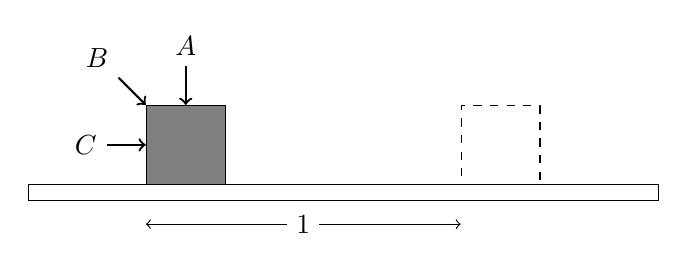
\begin{tikzpicture}
        \node[draw,fill=gray,anchor=south,rectangle,minimum size=1cm] (A) at (0,0) {};
        \draw[<-,thick] (A) -- ++(0,1) node[anchor=south] {$A$};
        \draw[<-,thick] (A) -- ++(-0.854,0.854) node[anchor=south east] {$B$};
        \draw[<-,thick] (A) -- ++(-1,0) node[anchor=east] {$C$};
        \draw (-2,0) rectangle (6,-0.2);
        \node[draw,dashed,anchor=south,rectangle,minimum size=1cm] (B) at (4,0) {};
        \draw[<->] (A.south west)++(0,-0.5) --  ++(4,0) node[midway,anchor=center,fill=white] {\SI{1}{\meter}};
    \end{tikzpicture}
    \end{center}
    \begin{choices}
        \wrongchoice{greatest for force $A$}
        \wrongchoice{greatest for force $B$}
      \correctchoice{greatest for force $C$}
        \wrongchoice{the same for all forces}
    \end{choices}
\end{question}
}

\element{cpo-mc}{
\begin{question}{cpo-ch04-q03}
    A unit used to measure power is the:
    \begin{choices}
        \wrongchoice{joule (\si{\joule})}
        \wrongchoice{newton per second (\si{\newton\per\second})}
        \wrongchoice{newton-meter (\si{\newton\meter})}
      \correctchoice{watt (\si{\watt})}
    \end{choices}
\end{question}
}

\element{cpo-mc}{
\begin{question}{cpo-ch04-q04}
    An automobile jack exerts a force of \SI{4 500}{\newton} to raise a car \SI{0.25}{\meter}.
    Which value is approximately the work done by the jack?
    \begin{multicols}{2}
    \begin{choices}
        \wrongchoice{\SI{0.00056}{\joule}}
      \correctchoice{\SI{1 100}{\joule}}
        \wrongchoice{\SI{4 500}{\joule}}
        \wrongchoice{\SI{18 000}{\joule}}
    \end{choices}
    \end{multicols}
\end{question}
}

\element{cpo-mc}{
\begin{question}{cpo-ch04-q05}
    A \SI{60}{\newton} block at rest at the bottom of a frictionless incline plane is pushed up the incline:
    \begin{center}
    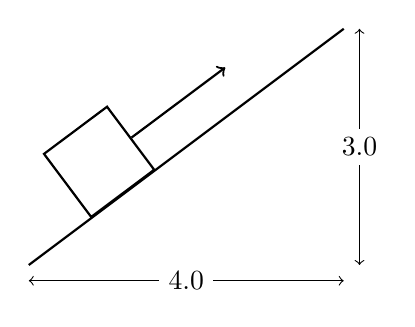
\begin{tikzpicture}
        \node[draw,thick,rotate=36.8,anchor=south,rectangle,minimum size=1cm] (A) at (36.8:1.5) {};
        \draw[thick,->] (A) -- ++(36.8:2);
        \draw[thick] (0,0) -- (4,3);
        \draw[<->] (0,-0.2) -- (4,-0.2) node[midway,anchor=center,fill=white] {\SI{4.0}{\meter}};
        \draw[<->] (4.2,0) -- (4.2,3) node[midway,anchor=center,fill=white] {\SI{3.0}{\meter}};
    \end{tikzpicture}
    \end{center}
    What is the amount of work done against gravity?
    \begin{multicols}{2}
    \begin{choices}
        \wrongchoice{\SI{0}{\joule}}
        \wrongchoice{\SI{20}{\joule}}
        \wrongchoice{\SI{60}{\joule}}
      \correctchoice{\SI{180}{\joule}}
    \end{choices}
    \end{multicols}
\end{question}
}

\element{cpo-mc}{
\begin{question}{cpo-ch04-q06}
    The action that would require no work to be done is:
    \begin{choices}
      \correctchoice{Holding a \SI{100}{\pound} object over your head.}
        \wrongchoice{Pushing a \SI{25}{\kilo\gram} box of books across the floor.}
        \wrongchoice{Pedaling a \SI{100}{\newton} bicycle up a small hill.}
        \wrongchoice{Lifting a balloon filled with air from the floor to a desktop.}
    \end{choices}
\end{question}
}

\element{cpo-mc}{
\begin{question}{cpo-ch04-q07}
    A \SI{2.2}{\kilo\gram} crate is pulled by a \SI{30}{\newton} force over a distance of \SI{5}{\meter}.
    What is the work done by pulling the crate?
    \begin{multicols}{2}
    \begin{choices}
        \wrongchoice{\SI{11}{\joule}}
        \wrongchoice{\SI{66}{\joule}}
      \correctchoice{\SI{150}{\joule}}
        \wrongchoice{\SI{330}{\joule}}
    \end{choices}
    \end{multicols}
\end{question}
}

\element{cpo-mc}{
\begin{question}{cpo-ch04-q08}
    When a force applied to an object causes the object to move in the direction of the force,
        the object acquires:
    \begin{choices}
      \correctchoice{energy}
        \wrongchoice{mechanical advantage}
        \wrongchoice{efficiency}
        \wrongchoice{friction}
    \end{choices}
\end{question}
}

\element{cpo-mc}{
\begin{question}{cpo-ch04-q09}
    Running up a flight of stairs, Maria generates \SI{450}{\watt} of power.
    If it takes her \SI{6}{\second} to go up the stairs,
        which is the amount of work she does running up the stairs?
    \begin{multicols}{2}
    \begin{choices}
        \wrongchoice{\SI{0.013}{\joule}}
        \wrongchoice{\SI{75}{\joule}}
        \wrongchoice{\SI{450}{\joule}}
      \correctchoice{\SI{2 700}{\joule}}
    \end{choices}
    \end{multicols}
\end{question}
}

\element{cpo-mc}{
\begin{question}{cpo-ch04-q10}
    Jasmine, who weighs \SI{400}{\newton}, moves up a \SI{5.0}{\meter} climbing wall in \SI{15}{\second}.
    Which is the amount of power generated by Jasmine as she climbs the wall?
    \begin{multicols}{2}
    \begin{choices}
      \correctchoice{\SI{130}{\watt}}
        \wrongchoice{\SI{2 000}{\watt}}
        \wrongchoice{\SI{6 000}{\watt}}
        \wrongchoice{\SI{30 000}{\watt}}
    \end{choices}
    \end{multicols}
\end{question}
}

\element{cpo-mc}{
\begin{question}{cpo-ch04-q11}
    If \SI{60}{\joule} of work are required to lift the \SI{10}{\newton} object \SI{5.0}{\meter} as shown in the diagram below.
    \begin{center}
    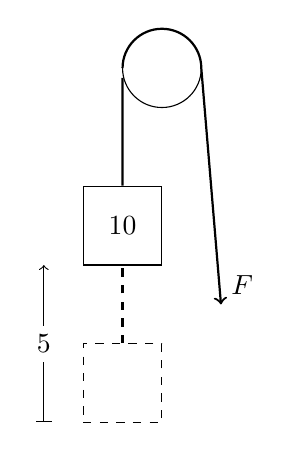
\begin{tikzpicture}
        \node[draw,dashed,rectangle,minimum size=1cm] (A) at (0,0) {};
        \node[draw,rectangle,minimum size=1cm] (B) at (0,2) {\SI{10}{\newton}};
        \node (P) at (0,4) { };
        \draw[thick,dashed] (A) -- (B);
        \draw[thick,->] (B) -- (P) arc(180:0:0.5) -- ++(0.25,-3) node[anchor=south west] {$F$};
        \draw[thin] (P) arc(180:360:0.5);
        \draw[|->] (-1.0,-0.5) -- (-1.0,1.5) node[midway,anchor=center,fill=white] {\SI{5}{\meter}};
    \end{tikzpicture}
    \end{center}
    Which is the work done in overcoming friction as the weight is lifted?
    \begin{multicols}{2}
    \begin{choices}
      \correctchoice{\SI{10}{\joule}.}
        \wrongchoice{\SI{50}{\joule}.}
        \wrongchoice{\SI{60}{\joule}.}
        \wrongchoice{\SI{300}{\joule}.}
    \end{choices}
    \end{multicols}
\end{question}
}

\element{cpo-mc}{
\begin{question}{cpo-ch04-q12}
    The diagram below shows a \SI{20}{\newton} force being applied to pull a \SI{5}{\kilo\gram} object up a hill at a constant speed.
    \begin{center}
    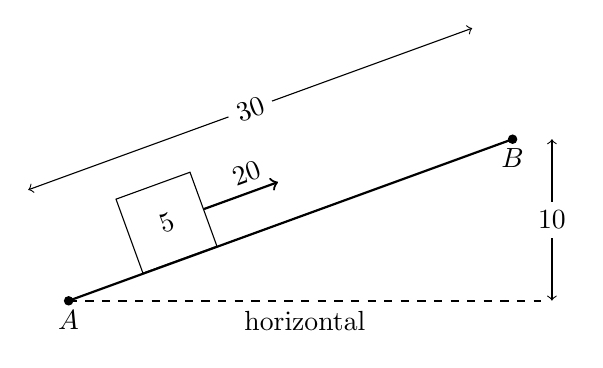
\begin{tikzpicture}
        %% Ramp
        \draw[thick] (0,0) -- (20:6);
        %% A and B Label
        \draw[fill] (20:0) circle  (1.5pt) node[anchor=north] {$A$};
        \draw[fill] (20:6) circle  (1.5pt) node[anchor=north] {$B$};
        %% length
        \draw[<->] (20:6) ++(0:0.5) -- ++(270:2.05) node[pos=0.5,anchor=center,fill=white] {\SI{10}{\meter}};
        \draw[<->] (0,0) ++(110:1.5) -- ++(20:6) node[pos=0.5,anchor=center,rotate=20,fill=white] {\SI{30}{\meter}};
        %% Block
        \node[draw,rectangle,minimum size=1cm,rotate=20,anchor=south west] (B) at (20:1) {\SI{5}{\kilo\gram}};
        \draw[thick,->] (B.east) -- ++ (20:1) node[pos=0.66,anchor=south,rotate=20] {\SI{20}{\newton}};
        %% Horizontal
        \draw[dashed,thick] (0:0) -- (0:6) node[pos=0.5,anchor=north] {horizontal};
    \end{tikzpicture}
    \end{center}
    Which is the amount of work that best represents the work done against in moving the object from point $A$ to point $B$?
    \begin{multicols}{2}
    \begin{choices}
        \wrongchoice{\SI{100}{\joule}}
      \correctchoice{\SI{200}{\joule}}
        \wrongchoice{\SI{500}{\joule}}
        \wrongchoice{\SI{600}{\joule}}
    \end{choices}
    \end{multicols}
\end{question}
}

\element{cpo-mc}{
\begin{question}{cpo-ch04-q13}
    Jordan lifts a \SI{100}{\kilo\gram} barbell from the floor to a height of \SI{2.0}{\meter} in \SI{1.5}{\second}.
    Which best represents the amount of power generated by Jordan?
    \begin{multicols}{2}
    \begin{choices}
        \wrongchoice{\SI{130}{\watt}}
        \wrongchoice{\SI{200}{\watt}}
      \correctchoice{\SI{1 310}{\watt}}
        \wrongchoice{\SI{1 960}{\watt}}
    \end{choices}
    \end{multicols}
\end{question}
}

\element{cpo-mc}{
\begin{question}{cpo-ch04-q14}
    An electrical water heater raises the temperature of water by adding \SI{8 000}{\joule} of energy to the water in \SI{40}{\second}.
    Which best represents the minimum amount of power that must be supplied to the heater?
    \begin{multicols}{2}
    \begin{choices}
        \wrongchoice{\SI{0.005}{\watt}}
      \correctchoice{\SI{200}{\watt}}
        \wrongchoice{\SI{3 200}{\watt}}
        \wrongchoice{\SI{320 000}{\watt}}
    \end{choices}
    \end{multicols}
\end{question}
}

\element{cpo-mc}{
\begin{question}{cpo-ch04-q15}
    The simple machine that operates as a ramp that curves around a shaft is a:
    \begin{choices}
        \wrongchoice{rope and pulley system}
      \correctchoice{screw}
        \wrongchoice{lever}
        \wrongchoice{gear}
    \end{choices}
\end{question}
}

\element{cpo-mc}{
\begin{question}{cpo-ch04-q16}
    In a theoretical machine, work output:
    \begin{choices}
        \wrongchoice{can be calculated by dividing output distance by output force.}
        \wrongchoice{is always greater than the work input.}
      \correctchoice{can be calculated by multiplying output force by output distance.}
        \wrongchoice{is always less than the work input.}
    \end{choices}
\end{question}
}

\element{cpo-mc}{
\begin{question}{cpo-ch04-q17}
    All of the following are considered to be simple machines \emph{except}:
    \begin{multicols}{2}
    \begin{choices}
        \wrongchoice{scissors}
      \correctchoice{a bicycle}
        \wrongchoice{a jackknife.}
        \wrongchoice{a see-saw.}
    \end{choices}
    \end{multicols}
\end{question}
}

\element{cpo-mc}{
\begin{question}{cpo-ch04-q18}
    The force directed along the ropes of a rope and pulley system is called:
    \begin{choices}
        \wrongchoice{thread.}
        \wrongchoice{lead.}
        \wrongchoice{mechanical advantage.}
      \correctchoice{tension.}
    \end{choices}
\end{question}
}

\element{cpo-mc}{
\begin{question}{cpo-ch04-q19}
    The fixed point around which levers rotate is called the:
    \begin{multicols}{2}
    \begin{choices}
        \wrongchoice{input arm.}
        \wrongchoice{output arm.}
      \correctchoice{fulcrum.}
        \wrongchoice{lever arm.}
    \end{choices}
    \end{multicols}
\end{question}
}

\element{cpo-mc}{
\begin{question}{cpo-ch04-q20}
    Talia pulls her younger brother in a wagon \SI{30}{\meter} to the top of a ramp \SI{3}{\meter} high.
    If the ramp is frictionless,
        which value best represents the mechanical advantage of this ramp?
    \begin{multicols}{4}
    \begin{choices}
        \wrongchoice{\num{0.10}}
      \correctchoice{\num{10}}
        \wrongchoice{\num{27}}
        \wrongchoice{\num{33}}
    \end{choices}
    \end{multicols}
\end{question}
}

\element{cpo-mc}{
\begin{question}{cpo-ch04-q21}
    The mechanical advantage of a lever is the ratio of the:
    \begin{choices}
      \correctchoice{length of the input arm to length of the output arm.}
        \wrongchoice{length of the output arm to the distance of the output arm.}
        \wrongchoice{input force to the output force.}
        \wrongchoice{input force to the distance the object moves.}
    \end{choices}
\end{question}
}

%\element{cpo-mc}{
%\begin{question}{cpo-ch04-q22}
%    If the top gear in each picture makes one complete turn,
%        which bottom gear makes the greatest number of turns?
%    \begin{center}
%    \begin{tikzpicture}
%        %% NOTE: TODO: draw tikz
%    \begin{tikzpicture}
%    \end{center}
%    \begin{multicols}{4}
%    \begin{choices}[o]
%        \wrongchoice{$A$}
%        \wrongchoice{$B$}
%        \wrongchoice{$C$}
%      \correctchoice{$D$}
%    \end{choices}
%    \end{multicols}
%\end{question}
%}

%\element{cpo-mc}{
%\begin{question}{cpo-ch04-q23}
%    The diagram illustrates a rope and pulley system being used
%        to raise a \SI{15}{\newton} weight:
%    \begin{center}
%    \begin{tikzpicture}
%        %% NOTE: TODO: draw tikz
%    \begin{tikzpicture}
%    \end{center}
%    Which best represents the tension in the rope?
%    \begin{multicols}{2}
%    \begin{choices}
%      \correctchoice{\SI{5}{\newton}}
%        \wrongchoice{\SI{10}{\newton}}
%        \wrongchoice{\SI{15}{\newton}}
%        \wrongchoice{\SI{20}{\newton}}
%    \end{choices}
%    \end{multicols}
%\end{question}
%}

\element{cpo-mc}{
\begin{questionmult}{cpo-ch04-Q24}
    A simple machine will sometimes multiply your:
    \begin{multicols}{3}
    \begin{choices}
        \wrongchoice{work.}
      \correctchoice{force.}
        \wrongchoice{energy.}
    \end{choices}
    \end{multicols}
\end{questionmult}
}

\element{cpo-mc}{
\begin{question}{cpo-ch04-q25}
    If the output force of a lever is greater than the input force, the:
    \begin{choices}
      \correctchoice{length of the input arm is greater than the length of the output arm.}
        \wrongchoice{mechanical advantage of the lever is less than one.}
        \wrongchoice{mechanical advantage of the lever is equal to one.}
        \wrongchoice{length of the output arm is greater than the length of the input arm.}
    \end{choices}
\end{question}
}

%\element{cpo-mc}{
%\begin{question}{cpo-ch04-q26}
%    The diagram picture a pulley system using \num{7} supporting ropes
%    \begin{center}
%    \begin{tikzpicture}
%        %% NOTE: TODO: draw tikz
%    \begin{tikzpicture}
%    \end{center}
%    If the boy in the picture weighs \SI{140}{\pound},
%        which value best represents the force that the baby must exert
%        to lift the boy?
%    \begin{multicols}{2}
%    \begin{choices}
%        \wrongchoice{\SI{70}{\pound}}
%        \wrongchoice{\SI{35}{\pound}}
%      \correctchoice{\SI{20}{\pound}}
%        \wrongchoice{\SI{7}{\pound}}
%    \end{choices}
%    \end{multicols}
%\end{question}
%}

%\element{cpo-mc}{
%\begin{question}{cpo-ch04-q27}
%    The diagram shows a gear system:
%    \begin{center}
%    \begin{tikzpicture}[scale=0.8]
%        %% Gears
%        \draw[thick] \gearmacro{36}{2cm}{2.2cm}{5}{1};
%        %\draw[fill=white] (0cm,0) circle (1cm); 
%        \draw[thick,xshift=2.87cm] \gearmacro{12}{0.67cm}{0.89cm}{15}{1};
%        %\draw[fill=gray] (2.87cm,0) circle (0.67cm); 
%        %\draw[fill=white] (2.87cm,0) circle (0.34cm); 
%        \draw[thick,xshift=5.09cm] \gearmacro{24}{1.33cm}{1.53cm}{7.5}{1};
%        %\draw[fill=gray] (5.09cm,0) circle (1.33cm); 
%        %\draw[fill=white] (5.09cm,0) circle (0.67cm); 
%        %% Labels
%        %\draw (-2.4cm,0) arc(180:45:2.4cm) node[pos=0.66,anchor=south] {12 turns};
%    \end{tikzpicture}
%    \end{center}
%    If the input gear turns \num{12} times, the number of turns made by the output gear is:
%    \begin{multicols}{4}
%    \begin{choices}
%        \wrongchoice{\num{12}}
%      \correctchoice{\num{18}}
%        \wrongchoice{\num{24}}
%        \wrongchoice{\num{48}}
%    \end{choices}
%    \end{multicols}
%\end{question}
%}

\element{cpo-mc}{
\begin{question}{cpo-ch04-q28}
    A screw with a lead of \SI{0.80}{\milli\meter} and a circumference of \SI{24}{\milli\meter} is turned into a board using a screwdriver with a mechanical advantage of 4.
    The total theoretical mechanical advantage is:
    \begin{multicols}{4}
    \begin{choices}
        \wrongchoice{\num{1.3}}
        \wrongchoice{\num{3.0}}
        \wrongchoice{\num{4.8}}
      \correctchoice{\num{120}}
    \end{choices}
    \end{multicols}
\end{question}
}

\element{cpo-mc}{
\begin{question}{cpo-ch04-q29}
    Josephine slides a \SI{150}{\newton} box \SI{12}{\meter} up an incline plane.
    If the plane lifts the box \num{4} meters as she pushes with a \SI{60}{\newton} force,
        the work input done by Josephine is: 
    \begin{multicols}{2}
    \begin{choices}
        \wrongchoice{\SI{48}{\joule}.}
        \wrongchoice{\SI{600}{\joule}.}
      \correctchoice{\SI{720}{\joule}.}
        \wrongchoice{\SI{9 000}{\joule}.}
    \end{choices}
    \end{multicols}
\end{question}
}

\element{cpo-mc}{
\begin{question}{cpo-ch04-q30}
    The measure of how effective a machine is in using energy to do work is called:
    \begin{choices}
        \wrongchoice{work output.}
        \wrongchoice{transformation.}
        \wrongchoice{mechanical advantage.}
      \correctchoice{efficiency.}
    \end{choices}
\end{question}
}

\element{cpo-mc}{
\begin{question}{cpo-ch04-q31}
    Friction is a ``catch-all'' term for many processes that oppose:
    \begin{choices}
        \wrongchoice{heat.}
        \wrongchoice{wear.}
      \correctchoice{motion.}
        \wrongchoice{neither heat, wear nor motion}
    \end{choices}
\end{question}
}

\element{cpo-mc}{
\begin{question}{cpo-ch04-q32}
    As fuel burns in a jet engine, it releases \SI{40 000}{\joule} of energy.
    The energy can be used to do \SI{16 000}{\joule} of work.
    The efficiency of the engine is: 
    \begin{multicols}{2}
    \begin{choices}
        \wrongchoice{\SI{20}{\percent}.}
      \correctchoice{\SI{40}{\percent}.}
        \wrongchoice{\SI{60}{\percent}.}
        \wrongchoice{\SI{250}{\percent}.}
    \end{choices}
    \end{multicols}
\end{question}
}

\element{cpo-mc}{
\begin{question}{cpo-ch04-q33}
    The work output is \SI{500}{\joule} for a machine that is \SI{25}{\percent} efficient.
    %% NOTE: fixed typo
    The work input is:
    \begin{multicols}{2}
    \begin{choices}
        \wrongchoice{\SI{125}{\joule}.}
        \wrongchoice{\SI{1 000}{\joule}.}
      \correctchoice{\SI{2 000}{\joule}.}
        \wrongchoice{\SI{12 500}{\joule}.}
    \end{choices}
    \end{multicols}
\end{question}
}

\element{cpo-mc}{
\begin{question}{cpo-ch04-q34}
    An incandescent light bulb uses \SI{60}{\joule\per\second} of electrical energy.
    \emph{Due to heat loss}, the energy available for light is reduced to only \SI{6}{\joule\per\second}.
    If this bulb is used to keep eggs warm in an incubator,
        about how efficient is the light bulb at producing \emph{heat}?
    \begin{multicols}{2}
    \begin{choices}
        %% NOTE: I corrected incorrect answer
        \wrongchoice{\SI{10}{\percent}.}
        \wrongchoice{\SI{20}{\percent}.}
        \wrongchoice{\SI{60}{\percent}.}
      \correctchoice{\SI{90}{\percent}.}
    \end{choices}
    \end{multicols}
\end{question}
}

\element{cpo-mc}{
\begin{question}{cpo-ch04-q35}
    Luis lifts a \SI{500}{\newton} load in a wheelbarrow \SI{0.15}{\meter} by raising the handles of the wheelbarrow \SI{0.40}{\meter} with a \SI{200}{\newton} force.
    The amount of work used to overcome friction is:
    \begin{multicols}{2}
    \begin{choices}
      \correctchoice{\SI{5}{\joule}.}
        \wrongchoice{\SI{75}{\joule}.}
        \wrongchoice{\SI{80}{\joule}.}
        \wrongchoice{\SI{200}{\joule}.}
    \end{choices}
    \end{multicols}
\end{question}
}


\endinput

